\uuid{7Soh}
\exo7id{7284}
\titre{exo7 7284}
\auteur{mourougane}
\organisation{exo7}
\datecreate{2021-08-10}
\isIndication{false}
\isCorrection{false}
\chapitre{Géométrie affine euclidienne}
\sousChapitre{Géométrie affine euclidienne du plan}
\module{Géométrie}
\niveau{L2}
\difficulte{}

\contenu{
\texte{
Soit \(\mathcal{C}\) un cercle de centre \(O\) et de rayon \(r\), et 
soit \(P\) un point. Soit \(\mathcal{D}\) une droite passant par \(P\) et 
qui coupe \(\mathcal{C}\) en deux points \(A\) et \(B\). La \emph{puissance} 
du point \(P\) par rapport au cercle \(\mathcal{C}\) est le produit scalaire 
\(\vec{PA} \cdot \vec{PB}\).

\begin{center}
    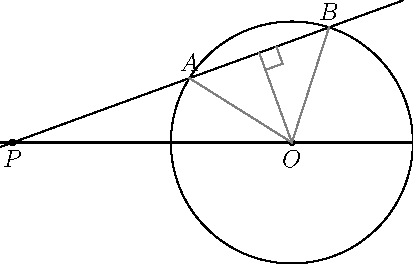
\includegraphics[scale=1]{images/pdf/7Soh-1.pdf}
\end{center}

% [[figure asymptote]]

%\begin{center}
%\begin{asy}
%size(7cm, 0);
%point O = (0, 0); dot("\(O\)", O, S);
%circle C0 = circle(O, 1.3); draw(C0);
%point P = (-3, 0); dot("\(P\)", P, S);
%line L0 = line(P, 0); draw(L0);
%line D0 = rotate(20, P) * L0; draw(D0);
%point[] AB = intersectionpoints(C0, D0);
%label("\(A\)", AB[0], N); label("\(B\)", AB[1], N);
%point Q = projection(D0) * O;
%draw(O--Q, gray); perpendicularmark(line(O, Q), D0, gray, quarter=3);
%draw(O--AB[0], gray); draw(O--AB[1], gray);
%\end{asy}
%\end{center}


Montrer que la puissance de \(P\) par rapport à \(\mathcal{C}\) est 
égale à \(OP^2 - r^2\). (Indication: utiliser le théorème de Pythagore.) 
Dépend-elle de la droite \(\mathcal{D}\) choisie?
}
}
